%% ICT2016.tex
\documentclass[conference]{IEEEtran}

\usepackage[utf8]{inputenc}
\usepackage[pdftex]{graphicx}
\usepackage{algorithm}
\usepackage{algorithmic}
\usepackage{subfigure}
\usepackage{url}

\ifCLASSINFOpdf
  % \usepackage[pdftex]{graphicx}
  % declare the path(s) where your graphic files are
  % \graphicspath{{../pdf/}{../jpeg/}}
  % and their extensions so you won't have to specify these with
  % every instance of \includegraphics
  % \DeclareGraphicsExtensions{.pdf,.jpeg,.png}
\else
  % or other class option (dvipsone, dvipdf, if not using dvips). graphicx
  % will default to the driver specified in the system graphics.cfg if no
  % driver is specified.
  % \usepackage[dvips]{graphicx}
  % declare the path(s) where your graphic files are
  % \graphicspath{{../eps/}}
  % and their extensions so you won't have to specify these with
  % every instance of \includegraphics
  % \DeclareGraphicsExtensions{.eps}
\fi
% graphicx was written by David Carlisle and Sebastian Rahtz. It is
% required if you want graphics, photos, etc. graphicx.sty is already
% installed on most LaTeX systems. The latest version and documentation
% can be obtained at: 
% http://www.ctan.org/tex-archive/macros/latex/required/graphics/
% Another good source of documentation is "Using Imported Graphics in
% LaTeX2e" by Keith Reckdahl which can be found at:
% http://www.ctan.org/tex-archive/info/epslatex/
%
% latex, and pdflatex in dvi mode, support graphics in encapsulated
% postscript (.eps) format. pdflatex in pdf mode supports graphics
% in .pdf, .jpeg, .png and .mps (metapost) formats. Users should ensure
% that all non-photo figures use a vector format (.eps, .pdf, .mps) and
% not a bitmapped formats (.jpeg, .png). IEEE frowns on bitmapped formats
% which can result in "jaggedy"/blurry rendering of lines and letters as
% well as large increases in file sizes.
%
% You can find documentation about the pdfTeX application at:
% http://www.tug.org/applications/pdftex


% correct bad hyphenation here
\hyphenation{op-tical net-works semi-conduc-tor}


\begin{document}
%
% paper title
% Titles are generally capitalized except for words such as a, an, and, as,
% at, but, by, for, in, nor, of, on, or, the, to and up, which are usually
% not capitalized unless they are the first or last word of the title.
% Linebreaks \\ can be used within to get better formatting as desired.
% Do not put math or special symbols in the title.
\title{Multichannel Cross-Layer Routing for Sensor Networks}


% author names and affiliations
% use a multiple column layout for up to three different
% affiliations
\author{\IEEEauthorblockN{Noradila Nordin}
\IEEEauthorblockA{
University College London\\
%Electronic and Electrical Engineering Department\\ University College London\\ 
%London, WC1E 7JE\\
Email: noradila.nordin.12@ucl.ac.uk}
\and
\IEEEauthorblockN{Richard G Clegg}
\IEEEauthorblockA{Imperial College London\\
Email: richard@richardclegg.org}
\and
\IEEEauthorblockN{Miguel Rio}
\IEEEauthorblockA{University College London\\
Email: miguel.rio@ucl.ac.uk}}

% make the title area
\maketitle

% As a general rule, do not put math, special symbols or citations
% in the abstract
\begin{abstract}
%The abstract goes here.
This paper proposes a new decentralised multi-channel tree building protocol with a centralised controller for the Internet of Things. The protocol alleviates the effect of interference which results in improved network efficiency and stability, and link reliability. The proposal takes into account all available channels to utilise the spectrum and aims to use the spectrum efficiently by transmitting on several channels. The protocol detects which channels suffer interference and changes away from those channels. The algorithm for channel selection is a two-hop colouring protocol that reduces the chances of nearby nodes to transmit on the same channel. All nodes are battery operated except for the low power border router (LPBR). This enables a centralised channel switching process at the LPBR. The protocol is built based on the routing protocol for low power and lossy networks (RPL). In its initial phase, the protocol uses RPL's standard topology formation to create an initial working topology and then seeks to improve this topology by switching channels. The implementation and evaluation of the protocol is performed using the Contiki framework. The experimental results demonstrate an increased resilience to interference and significant higher throughput making better use of the total available spectrum and link stability.
\end{abstract}
% no keywords




% For peer review papers, you can put extra information on the cover
% page as needed:
% \ifCLASSOPTIONpeerreview
% \begin{center} \bfseries EDICS Category: 3-BBND \end{center}
% \fi
%
% For peerreview papers, this IEEEtran command inserts a page break and
% creates the second title. It will be ignored for other modes.
\IEEEpeerreviewmaketitle

\section{Introduction}
\label{sec:introduction}
Wireless Sensor Networks (WSN) play a major role in the Internet of Things to enable and control groups of sensors to communicate over the Internet. This leads to a range of applications and services to be easily accessible.
%Wireless Sensor Networks (WSN) are the IoT networks that 
WSNs consist of sensor nodes that typically use low power radios such as IEEE 802.15.4, a relatively short range transmission standard radio technology in the 2.4 GHz band. The standard allows transmission to occur on several different channels within this band \cite{ieee802.15.4}. Unfortunately, the channels used by this technology often suffer interference \cite{Boano:2010:MSM:2127940.2127963, ieeeCompare}, for example, from Wi-Fi \cite{ieee_2012, wu} and Bluetooth. Sensor networks have to contend with an increasing number of devices that cause this wireless interference. Organising the network topology around this interference becomes an enabler for increasing transmission efficiency at a smaller energy cost. WSNs need to be able to operate reliably in the presence of such interference. It is important to minimise energy costs in these networks since deployments can be for weeks, months or longer.

Multichannel communication in wireless networks can alleviate the effects of interference which, as a result, can improve the network efficiency and stability, link reliability and minimise latency \cite{watteyne}. It also enables communication between physically proximate nodes to occur simultaneously without the risk of collision when the communicating nodes use different channels. However, not all channels are free from interference; thus, there is a gain to hop to another channel when the quality of the channel deteriorates. Two commonly used types of channel hopping \cite{watteyne} are blind channel hopping and whitelisting. In blind channel hopping, nodes choose from all available channels. 
Whitelisting, on the other hand, gives a set list of channels that avoids those that are known to commonly suffer interference.
Many studies make use of channel whitelisting such as in Chrysso \cite{chrysso} and MiCMAC\cite{micmac}.

Note that potentially Chrysso and MiCMAC could use all available channels.
However, they do not have a mechanism to check the channel condition before using it for packet transmission. MiCMAC sees its performance degraded when using more than 4 channels, thus the decision on specifying 4 channels to be included in their experiment. 
MiCMAC uses a different channel chosen at random each time it wakes up.
It might require several wake up periods which is time consuming, before a clear channel is found from the 16 channels, to deliver the packet.  
Chrysso on the other hand, switches the affected nodes to a new set of channels upon detecting interference which entails frequent channel switching if all channels are to be considered.

It is clear that it is impossible to find a single channel guaranteed free from interference and there is no consensus on the best channel to use. Our work takes into account all available channels to utilise the spectrum and checks the condition of the channels before hopping to avoid those channels with interference. Several previous studies have developed a multichannel MAC layer but, despite the potential benefits none are yet widely implemented in real world deployments.

This paper presents a Multichannel Cross-Layer Routing Protocol (MCRP) which consists of two main parts; a centralised intelligence at LPBR, and decentralised nodes. LPBR implements a two-hop colouring algorithm to avoid interference between physically proximate nodes trying to communicate on the same channel. The information on channel interference and network topology from the lower layer is made available to the application layer. This allows the centralised controller (LPBR) to have an overall view of the system to make decisions at the network and MAC layers about which channels nodes should listen on. The system is fail safe in the sense that the WSN functions if the central system which assigns channels fails temporarily or permanently.

We implement MCRP in Contiki \cite{contiki}, an open source operating system for WSNs and evaluate the protocol in Contiki network simulator, Cooja \cite{cooja}. 
We demonstrate that MCRP avoids channels with interference which greatly reduces the effects of interference on the network.

The rest of the paper is organised as follows: Section \ref{sec:relatedwork} presents related work to multichannel protocols. Section \ref{sec:multichannel} describes the key idea of our proposed protocol, the high-level design, and the implementation of the protocol in Contiki. We describe and evaluate the experimental results in Section \ref{sec:evaluation}. Finally, we conclude in Section \ref{sec:conclusion}.


\section{Related Work}
\label{sec:relatedwork}
Radio duty cycling mechanisms can be classified into two categories; synchronous and asynchronous systems. A synchronous system is a system that requires a tight time synchronisation between the nodes. It uses time-scheduled communication where the network clock needs to be periodically synchronised in order for the nodes not to drift in time. Asynchronous systems on the other hand, do not require synchronisation but instead is a sender or receiver initiated communication. In asynchronous systems the nodes are able to self-configure without time synchronisation and this can have advantages. There are many studies done in multichannel for both categories. Multichannel synchronous protocols include MC-LMAC \cite{mc-lmac}, Y-MAC \cite{y-mac}, and TSCH \cite{tsch}. Multichannel asynchronous protocols such as MuChMAC \cite{muchmac}, Chrysso \cite{chrysso}, MiCMAC \cite{micmac} and our protocol are independent of time slot and synchronisation. 

MiCMAC \cite{micmac} is a ContikiMAC \cite{contikimac} channel hopping variant. ContikiMAC was proved to be efficient in \cite{micmac,orpl} for a single channel. In MiCMAC, on every wakeup cycle, the channel is periodically switched according to a pseudo-random sequence. Chrysso \cite{chrysso} is a multichannel protocol for data collection applications. The nodes are organised into parent-children groups where each parent-children uses two channels for transmitting and receiving packets. MCRP also uses two separate channels as in Chrysso. In Chrysso, both parent and children nodes can hop to another channel when interference is detected based on the channel switching policies. Chrysso functionality comprises a set of channel switching policies that interface to both the MAC layer and the network layer. 

MiCMAC and Chrysso are fully distributed and allow the nodes to self configure and change to another channel when interference happens. The channels that the protocols can use are fixed to a subset of whitelisted channels. MiCMAC and Chrysso could use all channels, however, they do not have a mechanism for channel quality checking before a channel is chosen. It would be time consuming before it could find the interference free channel. This contrasts with our protocol where we are able to produce real time channel selection decisions by considering all available channels to be used in transmissions without blacklisting any of them. 

In order to maximise the use of multichannel in improving packet delivery, routing topology plays a big role in providing an optimised routing tree to the network that is scalable and energy efficient. There have been many studies on routing protocol such as LEACH \cite{leach}, PEGASIS \cite{pegasis}, CTP \cite{ctp}, and RPL \cite{winter2012rpl}. Recent multichannel protocols such as MiCMAC is compatible with RPL as the routing protocol. Chrysso uses Contiki collect which is a CTP-like data collection protocol in Contiki. Chrysso is restricted to only data collection networks. We choose to use RPL as it is the standard for IPv6 routing in low power and lossy networks. RPL \cite{winter2012rpl, routingmetrics, mrhof} is a gradient based routing protocol forming any-to-any routing for low power IPv6 networks. Our protocol makes use of RPL topology formation and improves on the channels of the nodes in the topology.

\section{Multichannel Cross-Layer Routing Protocol}
\label{sec:multichannel}

Multichannel Cross-Layer Routing Protocol (MCRP) concentrates on finding channels for nodes that are free from or have low interference. It allows the allocation of these channels in a way likely to minimise the chances of nodes which are physically near to communicate on the same channel. Hence, it reduces cross interference between different pairs of nodes.

\subsection{Overview}

The design of the multichannel protocol is based on several crucial observations:
\begin{itemize}
\item Channel assignment - Sensors have limited memory and battery capabilities. In order to maximise the sensors lifetime, a centralised LPBR that has larger memory and fully powered is used for decision making. LPBR has complete knowledge of the topology which enables it to make good channel assignment decisions based on a two-hop colouring algorithm.

\item Interference - External interference cannot be predicted, thus channels cannot be allocated beforehand as it varies over time and locations. It is impossible to determine a single channel that is free from interference at any location. Our protocol checks the channel condition each time before deciding on a channel change to reduce interference and maximise throughput.

\item Frequency diversity - Multichannel increases the robustness of the network towards interference. However, applying multichannel to the existing RPL may hinder detection of new nodes and cause problems for maintaining the RPL topology. We overcome this problem by two mechanisms.  Existing nodes maintain a table of the channels on which their neighbours listen and use unicast to contact those nodes.  New nodes listen on a Contiki default channel (26) and when connecting search through all channels. As in RPL, periodically all nodes broadcast RPL control messages on the default channel in an attempt to contact new nodes.
%Frequency diversity - Multichannel increases the robustness of the network towards interference. However, applying multichannel to the existing RPL may hinder neighbour detection and RPL processes to maintain the network topology as it does not switch to the correct channel. 
%We overcome this problem by enabling both broadcast (on a default channel), and unicast in neighbour detection and RPL control messages. 
%We overcome this problem in two ways.  Nodes new to the network listen on a default channel (26) but scan through all channels to contact the network.  As in RPL, existing nodes periodically broadcast the RPL control messages on the default channel in an attempt to contact nodes that have not yet joined the network. The control messages are sent as unicast for known neighbours channels.

%\item RPL - RPL messages are sent through unicast when the neighbours are known and broadcast in the default Contiki channel 26 in order to reduce unnecessary transmitting in broadcast. By sending a broadcast on only one channel on which the new neighbours are going to start, the nodes can be discovered and the channel change processes can be performed. 
%In multichannel, sending a broadcast on every channels would waste the bandwidth. RPL messages are instead sent through unicast when the neighbours are known and broadcast in the default Contiki channel 26 in order to reduce unnecessary transmitting in broadcast. By sending a broadcast on only one channel on which the new neighbours are going to start, the nodes can be discovered and the channel change processes can be performed. 

%\item Topology - The topology could change according to the routing metric the way the usual RPL would work. The nodes can still change the parents as usual as all neighbours know each other new channels. The neighbours that are not part of the route do not probe the parent when making the channel decision. However, the neighbours are informed of any channel changes.

\end{itemize}

Our cross-layer multi-channel protocol focuses on the network and application layers. This allows channel assignment decisions to be made thoroughly without being limited by the low layer complexity. The channel assignment processes take place only after the topology tree has been formed by RPL and stabilised. The system has two parts: a central algorithm which is typically run by the LPBR and selects which channel each node should listen on; and a protocol which allows the network to communicate the channel change decision, probe the new channel and either communicate the success of the change or fall back to the previous channel. 

\subsection{Channel Selection Strategy}

One main advantage of the system we propose is generality. Any algorithm can be used at the LPBR to assign channels. In this paper we use a two-hop colouring algorithm to select a channel to be assigned to a node.
The two-hop colouring algorithm attempts to ensure that nearby nodes do not communicate on the same channel and risk interfering with each other. The protocol is inspired by the graph colouring problems \cite{graphColouring}. The core idea is that no node should use the same listening channel as a neighbour or a neighbour of a neighbour (two hops).
This allows fair load balancing on the channels and reduces channel interference that could occur when two nearby nodes transmit together on the same channel. The nodes used in this paper have a transmission range of approximately 20-30 metres indoors and 75-100 metres outdoors \cite{telosb-datasheet}. It could be the case that many nodes in a sensor network are in the transmission range of each other and potentially interfered with.
 
All nodes are initialised to channel 26 which is the common default channel for Contiki MAC layer since it often has fewer interference problems with Wi-Fi and other sources. The studies in \cite{chrysso, micmac, watteyne} use a set list of whitelisted channels in their experiments and have channel 26 in common. The usual RPL set up mechanism is used to exchange control messages that are required to form an optimised topology before channel assignments can take place. The nodes will only be on the same channel once during the initial setup.  
	
In the two-hop colouring algorithm, the LPBR chooses a node to which it will assign a channel to listen on. The selection is random (from channels 11 to 26) based on the full range available \cite{ieee802.15.4}. The protocol checks neighbours and neighbours of neighbours to see if any of those are listening on this channel already. If any are, a new channel is picked from the remaining list of available channels. If the LPBR has knowledge of existing bad channels then those channels can be blacklisted.  Knowledge of channel interference which is gained by probing can be used to decide that a channel should not be used. If a channel is found then the channel switching protocol is triggered. If no channel can be found meeting these conditions, the current channel is kept.  

The node selection algorithm must only attempt one channel change at a time to ensure probing is done on the correct new channel and for the node to finalise the channel to be used before another node attempts a channel change.
The protocol ascertains that the channel change attempt will always result in a message returned to the LPBR either confirming the new channel or announcing a reversion to the old channel. Until one or other of these happens, no new channel change will be made to enable the neighbours transmitting on the correct channel.

\subsection{Channel Switching}
\label{sec:channelswitch}

\begin{figure}
\centering
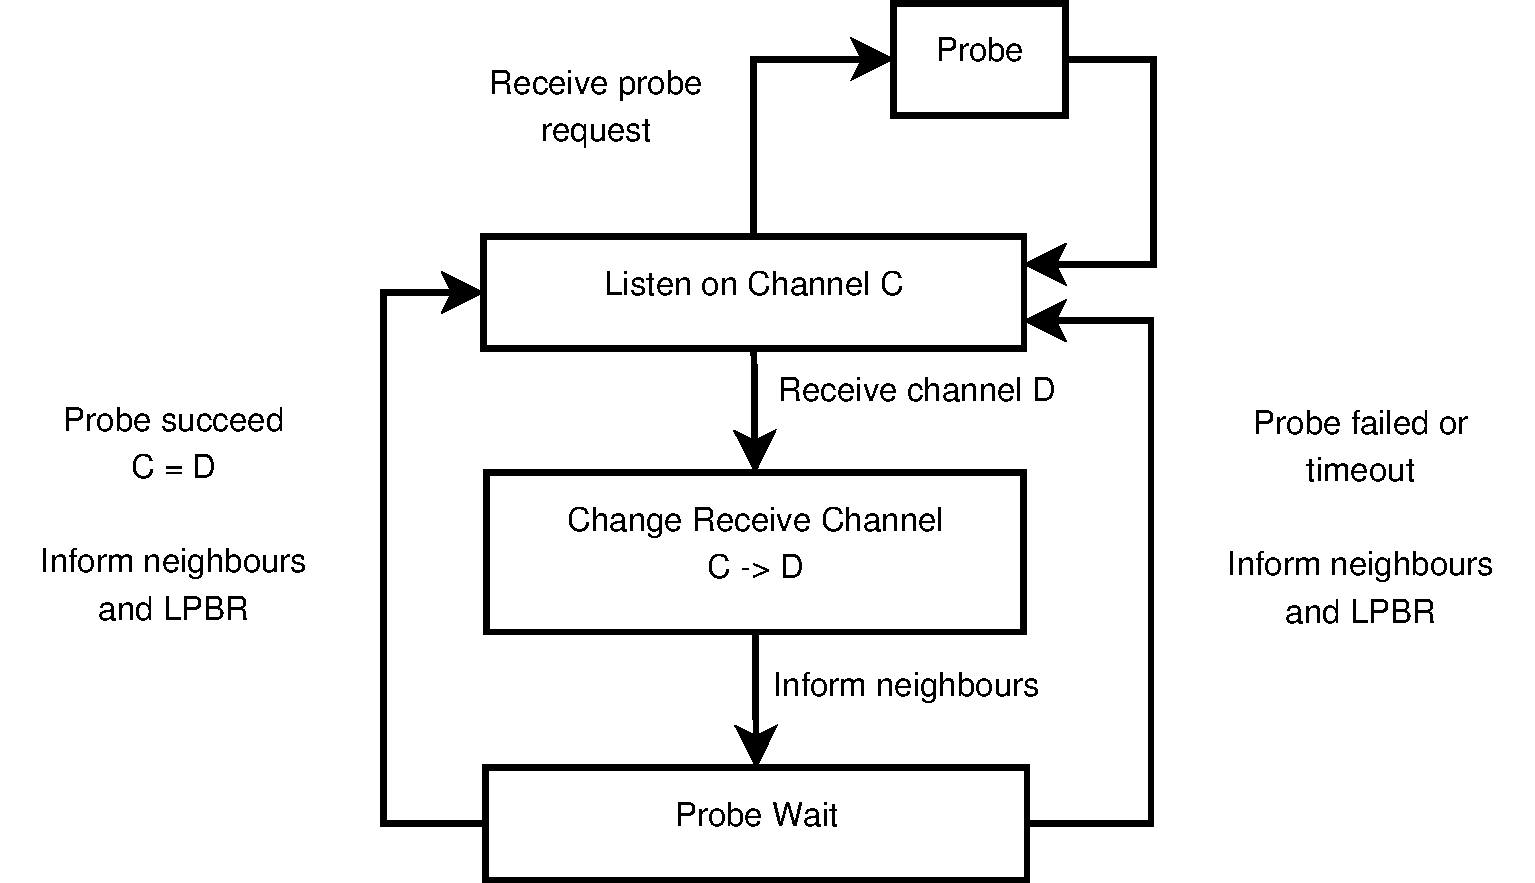
\includegraphics[width=3.5in]{Diagram1.pdf}
\caption{Channel switching processes}
\label{fig_sim}
\end{figure}

Figure \ref{fig_sim} shows the state machine for the channel switching protocol.
As explained in the previous section, a choice of a new channel by the channel selection protocol causes a change channel message to be sent to the appropriate node. 
Upon receiving a channel change message, a node $N$ stores its current channel $C$ and communicates to all its neighbours the new channel $D$ that it wishes to change to. Those neighbours will update their neighbour tables to ensure that they now send to node $N$ on channel $D$.  The node $N$ begins the channel quality checking process with each neighbour in turn by sending them a probe request. If this process fails for any neighbour then the node reverts to channel $C$. If all channel quality checks succeed, the node $N$ will listens on channel $D$. In both cases, node $N$ informs its neighbours of the decision to channel $C$ or $D$ and informs the LPBR of the channel checking results. The channel checking process uses probe packets that might interfere with other transmissions temporarily. However, it is important to emphasise that the network remains fully functional and connected at all stages of this protocol.

\subsection{Channel Quality Checking}
\label{sec:channelquality}

The channel quality checking is invoked each time a node changes channel after receiving a message from the LPBR. A node $N$ changing to channel $D$ informs all neighbours in turn, of the new channel $D$ it will be listening on as described in the previous section. It then enters the \emph{Probe Wait} state and begins channel quality checking with each tree neighbour in turn. In describing the channel quality checking process, it is worth emphasising the  distinction between neighbours and tree neighbours. Node neighbours are all nodes that a given node knows it could transmit to. Tree neighbours are the nodes that a node does transmit to through the topology formed by the RPL protocol. 

In the \emph{Probe Wait} state, node $N$ sends a \emph{Probe} message to each neighbour in turn. The neighbours respond to the message by sending eight packets to $N$ on the new channel $D$. 
The buffer can accommodate eight packets at a time. As the packets might not be sent immediately due to wakes up and collisions, sending more packets would have the risk of being dropped. 
The condition of the channel is further investigated through the number of retransmissions and packet collisions of the probing packets for accuracy of the channel condition. 

If the probing process times out (because of some communication failure) or the number of probe packets received is above a threshold (currently set to 16, including retransmissions and collisions) then node $N$ immediately exits \emph{Probe Wait} state and reverts to channel $C$ its previous channel. 


All neighbours are informed of the change back to channel $C$ and the LPBR is informed of the quality check failure with a summary of all probes received.
If, on the other hand, all channel quality checks succeed, the change to channel $D$ becomes permanent for node $N$ and it informs the LPBR of the results of the probing (numbers of packets received) and the channel change.

Probing is essential to make the channel change decision. It gives a quick overview of the channel condition based on the number of probing messages received. It is worth noting that probing is only done between the node and the tree neighbours. Neighbours that are not tree neighbours will not use the node as a route during their transmission thus, there is no need for probing to take place with those neighbours. However, the neighbours still need to know the channel value given that RPL control messages are sent to neighbours directly without using the routes.

\subsection{Reconnection Strategy}

RPL topology stability (using routing metric) remains the same in multi channel \cite{routingmetrics, winter2012rpl}.
%RPL topology could change according to the routing metric \cite{routingmetrics} the way the usual RPL would work \cite{winter2012rpl}. 
The nodes can still change the parents as usual as all neighbours know each other new channels. The neighbours that are not part of the route do not probe the parent when making the channel decision. However, the neighbours are informed of any channel changes.
This enables the topology to be optimised when communication fails and further improved through MCRP as the nodes have knowledge of the listening channels of all other nodes within the range. If a new node tries to join the topology, it sends a RPL control message through all channels as the listening nodes are unlikely to be on the default channel. The listening nodes send a broadcast on a default channel to discover new nodes (in Contiki default, new nodes will start on channel 26) and send RPL messages through unicast when the neighbours are known to reduce unnecessary transmissions in broadcast. New nodes and nodes which fall off the network can now rejoin on many potential channels. 
RPL makes use of trickle timers in order to reduce the number of overhead compared to the number of actual data packet by eliminating redundant RPL control messages. 
%The number of overhead is less than the actual data packet.


\section{Evaluation}
\label{sec:evaluation}
The performance of MCRP is compared against the standard ContikiMAC with RPL. The interference pattern obtained in \cite{radioBoano} is used. We analyse MCRP using an end-to-end packet delivery performance metric.

\subsection{Experimental Setup}
We evaluate the protocol in the  Cooja simulated environment with emulation of TMote sky nodes that feature the CC2420 transceiver, a 802.15.4 radio. The nodes run on IPv6, using UDP with standard RPL and 6LoWPAN protocols. The network consists of 31 nodes which are used to run the simulation where we have 1 border router node, 16 interference nodes, and 14 duty cycled nodes that act as UDP clients to send packets to LPBR spanning over 20-30 metres between each node. RPL border router is used as LPBR in order to move most processing decisions on a PC as it has more RAM and better processing capabilities than a sensor. TelosB has limited RAM and ROM of 10K bytes and 48K bytes of flash memory \cite{telosb-datasheet}. By using a border router, it allows channel changing to be decided in real time without draining the memory and battery on a sensor. The border router also acts as the root of the tree.

We simulated a controlled interference node that generates semi-periodic bursty interference to resemble a simplified Wi-Fi or Bluetooth transmitter on several channels at random. We use the interference model proposed in \cite{Boano:2010:MSM:2127940.2127963} to generate similar packet loss rate to the theoretical and real nodes values given in \cite{radioBoano}. The interference has two states, a clear state and an interference state. 
In the interference state, the interference node generates packets for a time that is uniformly distributed between $9/16$ seconds and $15/16$ seconds. In the clear state the interferer produces no packets and stays in this state for between $3/4 * \emph{clear\textunderscore time}$ and $5/4 * \emph{clear\textunderscore time}$ where \emph{clear\textunderscore time} refers to the rate of interference.
We use multiple channels interference in our simulation to show our hypothesis that our multichannel protocol can help avoid interference. We consider the scenario where ContikiMAC with RPL system is subject to interference on its channel after set up has successfully completed so the RPL set up is allowed to complete before interference begins.

We use an end-to-end packet delivery performance metric to evaluate MCRP. The transmission success rate is calculated from the sender to the receiver over multiple hops. We also look at the loss over time to observe the protocol performance in the presence of interference. We considered two multiple channels interference scenarios; (1) extreme and no interference rate on 8 channels each and (2) extreme, moderate, mild and no interference rate on 4 channels each. The interference channels are randomly chosen from the available 16 channels and the same interference channels and rates are used throughout the experiments. However, channel 26 is kept clear from interference in order to ensure RPL set up is unaffected. In scenario 1, we fixed the interference rate to extreme and no interference to observe the effect it has on channel changing decisions. In scenario 2, we vary the interference rate to observe how MCRP copes in deciding a channel when there is more interference than scenario 1 but with less interference intensity. 

We run the simulation for a duration of 45-60 minutes to send 210-560 packets. When the nodes are switched on for the first time, all nodes are initialised to channel 26, the default channel for Contiki MAC layer. RPL is allowed five minutes to set up (which is ample time). RPL topology is formed in a minute. We wait for another five minutes to allow trickle timer to double the interval length so that RPL control messages are not being sent frequently. We then let our multichannel protocol run for 25 minutes. In our 15 nodes simulation, our protocol takes 20-25 minutes to run the channel change set up. We allow another 5 minutes wait time if retransmissions happen. 
In a single channel simulation, all the nodes are changed to channel 22 after 5 minutes of RPL set up time. This allows RPL to have enough time to discover all nodes to form an optimised topology. The topology formation does not form completely if the interference node interferes from the beginning. The interference node starts sending packets to interfere after 3 minutes the system is switched on so that the interference channel is involved in the channel changes decision. We proved that our protocol tries to avoid changing to the interference channel through time out and probing failures. After 30 minutes, the client nodes will send a normal packet periodically every 30-60 seconds to LPBR. This is done in order to avoid collision of the nodes sending at the same time. 
The simulations are repeated ten times. In all plots, the mean value of the ten simulations is plotted with error bars corresponding to one standard deviation in either deviation to give a measure of repeatability. The plots are of the proportion of received packets (from 0\% to 100\%) against time where the loss is measured over the previous time period.  The x-value is shifted slightly left and right to prevent error bars overlapping.

\subsection{Packet loss rates with single channel RPL versus multi-channel}
The performance obtained in ContikiMAC with RPL (single channel) is compared with our protocol in terms of packet loss rate.
As described previously, levels of interference used (referred to as \emph{clear\textunderscore time} in \cite{Boano:2010:MSM:2127940.2127963})
vary among 100\% (no interference), 75\% (mild), 50\% (moderate) and 25\% (extreme) where the percentage is the ratio of the time the channel is clear for transmission.  All our tests have a common format: the RPL procedure is allowed to set up without interference in order not to bias subsequent tests.
Then the interferers begin to operate with a constant level (none, mild, moderate or extreme).

\begin{figure}
\centering
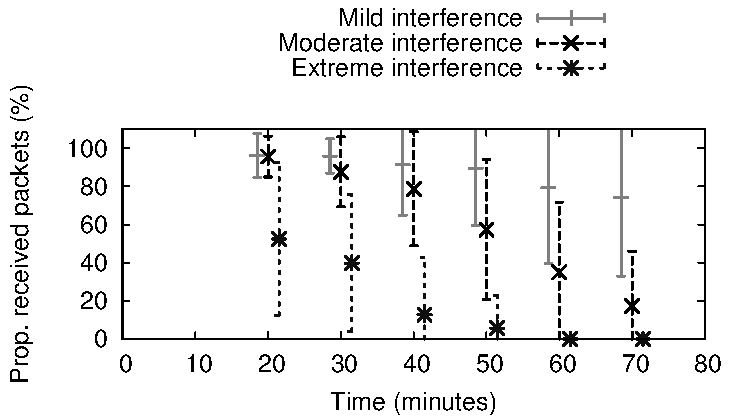
\includegraphics[width=0.45\textwidth]{experiments/single_channel.pdf}
\caption{Level of packet loss for mild, moderate and extreme interference levels using single channel}
\label{fig:interference}
\end{figure}

\begin{figure}
\centering
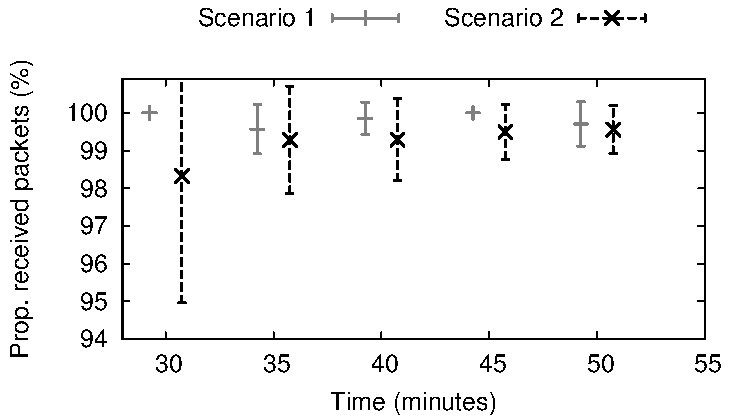
\includegraphics[width=0.45\textwidth]{experiments/multi_channel.pdf}
\caption{Level of packet loss for scenario 1 and scenario 2 using multi channel}
\label{fig:multi_interference}
\end{figure}

Figure \ref{fig:interference} shows the results for ContikiMAC with RPL protocol. It can be seen that the level of packet loss varies considerably between experiments (the error bars are always large). It can also be seen that even for mild interference there is considerable loss and this gets worse as time proceeds. In the extreme interference case the loss always goes up until no packets are received. For mild interference the system evolves until it is losing around 20\% of packets but this can increase.

For our new multiple channel protocol we consider two interference scenarios.
In scenario 1 half the channels (including the original channel) have no
interference at all and half the channels have extreme interference.
In scenario 2, four channels (including the original channel) have no
interference, four have mild, four moderate and four extreme interference.
Figure \ref{fig:multi_interference} shows multi channel results for these
two scenarios.  In scenario 1 the protocol performs extremely well, the packet loss is near zero and the protocol successfully detects channels with interference.
Scenario 2 has similar results as in scenario 1. The protocol does well at reducing the effects of interference and could detect moderate and mild interference.

In MiCMAC \cite{micmac}, it is stated that MiCMAC has a transmission success rate of 99\% when using four channels. However, when more than four channels are used (8 or 16 channels), MiCMAC performance degrades to approximately 88\% (16 channels) due to interference channels. The interference model that MiCMAC uses is different than ours. They compare the result with Chrysso where Chrysso has a transmission success rate of approximately 88\% for 4 and 8 channels and suffers greatly in the case of 16 channels with 60\% success rate.
Our protocol on the other hand, shows greatly reduced loss rate with any number of channels at approximately 99\%.

\subsection{Setup Overhead}
Obviously the system of changing channels and probing to see if a channel is free of interference introduces a certain amount of overhead into
the protocol. This takes the form of (a) extra messages passed and (b) extra time taken to set up. Default RPL on ContikiMAC for the topology considered in these experiments completed its set up using 276 packets. Our multi-channel protocol completed its set up in 716 packets, that is an overhead of 440 packets on top of RPL. 
This overhead comes from the channel changing messages to nodes and neighbours, probing messages, channel confirmation messages and acknowledgement packets which are required to ensure a thorough channel change decision.
However, it is worth mentioning that this is a one-off cost. This represents (in this experimental set up) approximately one hour of extra packets in the situation of a deployment that is meant to work for weeks or months.  In terms of set up time, our protocol begins to change channels only when the RPL set up process is complete (or at least stabilises). The set up time is 1154 seconds beyond the RPL set up time of 286 seconds. However, it should be noted that, in fact, our system remains fully functional and capable of sending packets during the set up so this set up overhead does not matter to data transmission.
Therefore we conclude that data sending costs (extra packets) of set up are negligible in the context of a deployment that will last more than a day. The extra set up time is also negligible within this context and furthermore does not degrade performance of the network during this set up phase.

\section{Conclusion}
\label{sec:conclusion}
We presented MCRP, a decentralised cross-layer protocol with a centralised controller. Our protocol mitigates the effect of interference by avoiding affected channels. It allows better spectrum usage by trying to move nearby nodes to listen on different channels using two-hop colouring algorithm. Our protocol provides feedback when a channel is subject to interference using a probing phase.
The results from the simulation showed that our protocol avoids channels with interference hence greatly reduced loss rates with negligible overhead. By reducing packet loss (hence retransmissions) and increasing the efficiency of spectrum usage, the multichannel system will be more energy efficient than single channel ContikiMAC with RPL over the lifetime of the system's deployment.

Future work is ongoing to develop the protocol. Deployment is underway on the Flocklab testbed \cite{flocklab}. Next we plan to improve the interference model we used to better replicate the real world environment. 
%The protocol will be tested against competing multi-channel protocols such as MiCMAC. We also plan to test our implementation on real hardware.  Finally we will allow nodes to update the LPBR on ongoing packet loss so that the network can continually respond to changes in congestion.



\section*{Acknowledgments}
Noradila Nordin is a King's Scholar sponsored by the Government of Malaysia.

\label{references}
%\nocite{*}
\bibliography{ICT2016}
\bibliographystyle{plain}

\end{document}